\documentclass[journal,12pt,twocolumn]{IEEEtran}

\usepackage{setspace}
\usepackage{gensymb}

\singlespacing


\usepackage[cmex10]{amsmath}

\usepackage{amsthm}

\usepackage{mathrsfs}
\usepackage{txfonts}
\usepackage{stfloats}
\usepackage{bm}
\usepackage{cite}
\usepackage{cases}
\usepackage{subfig}

\usepackage{longtable}
\usepackage{multirow}

\usepackage{enumitem}
\usepackage{mathtools}
\usepackage{steinmetz}
\usepackage{tikz}
\usepackage{circuitikz}
\usepackage{verbatim}
\usepackage{tfrupee}
\usepackage[breaklinks=true]{hyperref}
\usepackage{graphicx}
\usepackage{tkz-euclide}

\usetikzlibrary{calc,math}
\usepackage{listings}
    \usepackage{color}                                            %%
    \usepackage{array}                                            %%
    \usepackage{longtable}                                        %%
    \usepackage{calc}                                             %%
    \usepackage{multirow}                                         %%
    \usepackage{hhline}                                           %%
    \usepackage{ifthen}                                           %%
    \usepackage{lscape}     
\usepackage{multicol}
\usepackage{chngcntr}

\DeclareMathOperator*{\Res}{Res}

\renewcommand\thesection{\arabic{section}}
\renewcommand\thesubsection{\thesection.\arabic{subsection}}
\renewcommand\thesubsubsection{\thesubsection.\arabic{subsubsection}}

\renewcommand\thesectiondis{\arabic{section}}
\renewcommand\thesubsectiondis{\thesectiondis.\arabic{subsection}}
\renewcommand\thesubsubsectiondis{\thesubsectiondis.\arabic{subsubsection}}


\hyphenation{op-tical net-works semi-conduc-tor}
\def\inputGnumericTable{}                                 %%

\lstset{
%language=C,
frame=single, 
breaklines=true,
columns=fullflexible
}
\begin{document}


\newtheorem{theorem}{Theorem}[section]
\newtheorem{problem}{Problem}
\newtheorem{proposition}{Proposition}[section]
\newtheorem{lemma}{Lemma}[section]
\newtheorem{corollary}[theorem]{Corollary}
\newtheorem{example}{Example}[section]
\newtheorem{definition}[problem]{Definition}

\newcommand{\BEQA}{\begin{eqnarray}}
\newcommand{\EEQA}{\end{eqnarray}}
\newcommand{\define}{\stackrel{\triangle}{=}}
\bibliographystyle{IEEEtran}
\providecommand{\mbf}{\mathbf}
\providecommand{\pr}[1]{\ensuremath{\Pr\left(#1\right)}}
\providecommand{\qfunc}[1]{\ensuremath{Q\left(#1\right)}}
\providecommand{\sbrak}[1]{\ensuremath{{}\left[#1\right]}}
\providecommand{\lsbrak}[1]{\ensuremath{{}\left[#1\right.}}
\providecommand{\rsbrak}[1]{\ensuremath{{}\left.#1\right]}}
\providecommand{\brak}[1]{\ensuremath{\left(#1\right)}}
\providecommand{\lbrak}[1]{\ensuremath{\left(#1\right.}}
\providecommand{\rbrak}[1]{\ensuremath{\left.#1\right)}}
\providecommand{\cbrak}[1]{\ensuremath{\left\{#1\right\}}}
\providecommand{\lcbrak}[1]{\ensuremath{\left\{#1\right.}}
\providecommand{\rcbrak}[1]{\ensuremath{\left.#1\right\}}}
\theoremstyle{remark}
\newtheorem{rem}{Remark}
\newcommand{\sgn}{\mathop{\mathrm{sgn}}}
\providecommand{\abs}[1]{\left\vert#1\right\vert}
\providecommand{\res}[1]{\Res\displaylimits_{#1}} 
\providecommand{\norm}[1]{\left\lVert#1\right\rVert}
%\providecommand{\norm}[1]{\lVert#1\rVert}
\providecommand{\mtx}[1]{\mathbf{#1}}
\providecommand{\mean}[1]{E\left[ #1 \right]}
\providecommand{\fourier}{\overset{\mathcal{F}}{ \rightleftharpoons}}
%\providecommand{\hilbert}{\overset{\mathcal{H}}{ \rightleftharpoons}}
\providecommand{\system}{\overset{\mathcal{H}}{ \longleftrightarrow}}
	%\newcommand{\solution}[2]{\textbf{Solution:}{#1}}
\newcommand{\solution}{\noindent \textbf{Solution: }}
\newcommand{\cosec}{\,\text{cosec}\,}
\providecommand{\dec}[2]{\ensuremath{\overset{#1}{\underset{#2}{\gtrless}}}}
\newcommand{\myvec}[1]{\ensuremath{\begin{pmatrix}#1\end{pmatrix}}}
\newcommand{\mydet}[1]{\ensuremath{\begin{vmatrix}#1\end{vmatrix}}}
\numberwithin{equation}{subsection}
\makeatletter
\@addtoreset{figure}{problem}
\makeatother
\let\StandardTheFigure\thefigure
\let\vec\mathbf
\renewcommand{\thefigure}{\theproblem}
\def\putbox#1#2#3{\makebox[0in][l]{\makebox[#1][l]{}\raisebox{\baselineskip}[0in][0in]{\raisebox{#2}[0in][0in]{#3}}}}
     \def\rightbox#1{\makebox[0in][r]{#1}}
     \def\centbox#1{\makebox[0in]{#1}}
     \def\topbox#1{\raisebox{-\baselineskip}[0in][0in]{#1}}
     \def\midbox#1{\raisebox{-0.5\baselineskip}[0in][0in]{#1}}
\vspace{3cm}
\title{Assignment 2}
\author{K.A. Raja Babu}
\maketitle
\newpage
\bigskip
\renewcommand{\thefigure}{\theenumi}
\renewcommand{\thetable}{\theenumi}
Download all python codes from 
\begin{lstlisting}
https://github.com/ka-raja-babu/Matrix-Theory/tree/main/Assignment2/Codes
\end{lstlisting}
%
and latex-tikz codes from 
%
\begin{lstlisting}
https://github.com/ka-raja-babu/Matrix-Theory/tree/main/Assignment2
\end{lstlisting}
%
\section{Question No. 32}
Can you construct a quadrilateral $PQRS$ with $PQ$ = 3,$RS$ = 3,$PS$ = 7.5,$PR$ = 8 and $SQ$ = 4 ?
%

\section{Explanation}
Let us assume that:

\begin{align}
\vec{P} = \myvec{0\\0}, \vec{Q} = \myvec{a\\b}, \vec{R} = \myvec{c\\d},\vec{S} = \myvec{7.5\\0}
\end{align}

Then,
\begin{align}
\norm{\vec{Q}-\vec{P}}^2 = \norm{\vec{Q}}^2  = 3^2 =9 \quad \brak{\because \vec{P}=0} 
\\
\norm{\vec{S}-\vec{P}}^2 = \norm{\vec{S}}^2 = (7.5)^2 =56.25 \quad \brak{\because \vec{P}=0} 
\\
\norm{\vec{R}-\vec{P}}^2 = \norm{\vec{R}}^2 = 8^2 = 64 \quad \brak{\because \vec{P}=0} 
\end{align}

Now,
\begin{align}
\norm{\vec{Q}-\vec{S}}^2 &= ({\vec{Q}-\vec{S}})^T({\vec{Q}-\vec{S}})
\\
&= \vec{Q}^T\vec{Q}+\vec{S}^T\vec{S}-\vec{Q}^T\vec{S} - \vec{Q}^T\vec{S}
\\
&= \norm{\vec{Q}}^2 + \norm{\vec{S}}^2 - 2\vec{Q}^T\vec{S} \quad \brak{\because \vec{Q}^T\vec{S} = \vec{S}^T\vec{Q} } 
\\
&= 9 + 56.25 -2(7.5a) \quad \brak{\because \vec{Q}^T\vec{S} = 7.5a } 
\\
&= 65.25 - 15a
\end{align}

But,
\begin{align}
\norm{{\vec{Q}-\vec{S}}}^2=4^2=16 \quad \brak{\because Given}
\end{align}

Therefore,
\begin{align}
65.25 - 15a = 16
\\
\implies 15a = 49.25
\\
\implies a = 3.283
\end{align}

Now,
\begin{align}
\norm{\vec{Q}}^2  = a^2 + b^2 =3^2 =9
\\
\implies (3.283)^2 + b^2 =9
\\
\implies b^2 = -1.778
\\
\implies b = 1.33\iota
\end{align}

Similarly,
\begin{align}
\norm{\vec{R}-\vec{S}}^2 &= ({\vec{R}-\vec{S}})^T({\vec{R}-\vec{S}})
\\
&= \vec{R}^T\vec{Q}+\vec{S}^T\vec{S}-\vec{R}^T\vec{S} - \vec{R}^T\vec{S}
\\
&= \norm{\vec{R}}^2 + \norm{\vec{S}}^2 - 2\vec{R}^T\vec{S} \quad \brak{\because \vec{R}^T\vec{S} = \vec{S}^T\vec{R} } 
\\
&= 64 + 56.25 -2(7.5c) \quad \brak{\because \vec{Q}^T\vec{S} = 7.5c } 
\\
&= 120.25 - 15c
\end{align}

Again,
\begin{align}
\norm{{\vec{R}-\vec{S}}}^2=3^2=9 \quad \brak{\because Given}
\end{align}

Therefore,
\begin{align}
120.25 - 15c = 9
\\
\implies 15c = 111.25
\\
\implies c = 7.416
\end{align}

Now,
\begin{align}
\norm{\vec{R}}^2  = c^2 + d^2 =8^2 = 64
\\
\implies (7.416)^2 + d^2 = 64
\\
\implies d^2 = 9.00
\\
\implies d = 3
\end{align}

Therefore,vertices of quadrilateral $PQRS$ are as follows:
\begin{align}
\vec{P} = \myvec{0\\0}, \vec{Q} = \myvec{3.283\\1.33\iota}, \vec{R} = \myvec{7.416\\3},\vec{S} = \myvec{7.5\\0}
\end{align}
\\
But,value of $b$ comes imaginary which cannot be represented in Cartesian coordinate system.
\\
This implies that our assumption is wrong and there exists no real values of $b$ which satisfy these conditions. 
\\
Hence,quadrilateral $PQRS$ cannot be constructed with these values.
\\
Figure \ref{fig:quadrilateral} is plotted taking $b$ as 0 discarding its imaginary part ,which looks like a triangle not a quadrilateral.
\\
This plot clearly concludes that construction of quadrilateral $PQRS$ is not possible with these values.
\\
Plot of the quadrilateral $PQRS$ taking $b$ = 0 :
\numberwithin{figure}{section}
\begin{figure}[!ht]
\centering
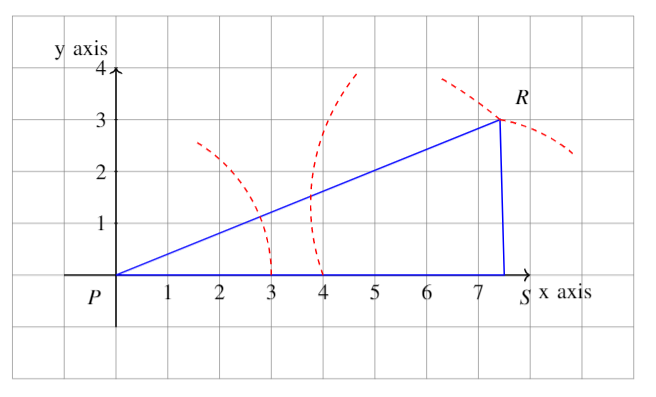
\includegraphics[width=\columnwidth]{Figure2}
\caption{Quadrilateral $PQRS$ when $b$ =0}
\label{fig:quadrilateral}	
\end{figure}
\end{document}
